\documentclass[preprint]{acmsiggraph}
\listfiles
\usepackage{amsmath,amssymb,multirow}
\graphicspath{{figures/}}

% -*- compile-command: "texify --pdf --quiet arapsfm.tex" -*-
 
%\newcommand{\aaron}[1]{ }
\newcommand{\aaron}[1]{\textcolor{red}{\bf [AH: #1]}}
\newcommand{\richard}[1]{\textcolor{blue}{\bf [R: #1]}}
\newcommand{\awf}[1]{\textcolor{magenta}{\bf [AWF: #1]}}

\newcommand{\vectwo}[2]{\left[\begin{array}{c} #1 \\ #2 \end{array} \right ]}
\newcommand{\mattwo}[4]{\left[\begin{array}{cc} #1 & #2 \\ #3 & #4 \end{array} \right ]}
\newcommand{\ba}{\mathbf{a}}
\newcommand{\bb}{\mathbf{b}}
\newcommand{\bc}{\mathbf{c}}
\newcommand{\mybf}{\mathbf{f}}
\newcommand{\bB}{\mathbf{B}}
\newcommand{\bS}{\mathbf{S}}
\newcommand{\bG}{\mathbf{G}}
\newcommand{\bI}{\mathbf{I}}
\newcommand{\bJ}{\mathbf{J}}
\newcommand{\bK}{\mathbf{K}}
\newcommand{\bk}{\mathbf{k}}
\newcommand{\bL}{\mathbf{L}}
\newcommand{\bU}{\mathbf{U}}
\newcommand{\bV}{\mathbf{V}}
\newcommand{\bF}{\mathbf{F}}
\newcommand{\bs}{\mathbf{s}}
\newcommand{\bT}{\mathbf{T}}
\newcommand{\bM}{\mathbf{M}}
\newcommand{\bn}{\mathbf{n}}
\newcommand{\bN}{\mathbf{N}}
\newcommand{\bW}{\mathbf{W}}
\newcommand{\bp}{\mathbf{p}}
\newcommand{\bq}{\mathbf{q}}
\newcommand{\br}{\mathbf{r}}
\newcommand{\bP}{\mathbf{P}}
\newcommand{\bx}{\mathbf{x}}
\newcommand{\bw}{\mathbf{w}}
\newcommand{\bv}{\mathbf{v}}
\newcommand{\bu}{\mathbf{u}}
\newcommand{\bell}{\mathbf{\ell}}

\newcommand{\bomegaa}{\mbox{\boldmath$\omega$}}
\newcommand{\wpreimage}{\mathbf{w}}
\newcommand{\bPi}{\mbox{\boldmath$\Pi$}}

\newcommand{\bbv}{\bar{\bv}}

\newcommand{\cI}{\mathcal{I}}
\newcommand{\cR}{\mathcal{R}}
\newcommand{\cN}{\mathcal{N}}
\newcommand{\cB}{\mathcal{B}}
\newcommand{\cV}{\mathcal{V}}
\newcommand{\cU}{\mathcal{U}}
\newcommand{\cE}{\mathcal{E}}
\newcommand{\cT}{\mathcal{T}}
\newcommand{\cC}{\mathcal{C}}
\newcommand{\cW}{\mathcal{W}}
\newcommand{\cP}{\mathcal{P}}
\newcommand{\cQ}{\mathcal{Q}}
\newcommand{\cG}{\mathcal{G}}

\newcommand{\E}[1]{E_{\text{\em #1}}}
\newcommand{\w}[1]{w_{\text{\em #1}}}


\def\Vtemplate{\cV_{\text{template}}}
\def\Vcore{\cV_{\text{core}}}

\def\eqref#1{(\ref{eq:#1})}
\def\Eqref#1{(Eq.~\ref{eq:#1})}
\def\Figref#1{Fig.~\ref{fig:#1}}


\def\grp#1{\textsf{#1}}


\pdfcompresslevel9

\TOGonlineid{629}
\TOGvolume{0}
\TOGnumber{0}
\TOGarticleDOI{1111111.2222222}
\TOGprojectURL{}
\TOGvideoURL{}
\TOGdataURL{}
\TOGcodeURL{}

\title{Deformable Mesh Animation from Single-View Video}

\makeatletter
\renewcommand{\@ACMpreprinttext}{SUBMISSION UNDER REVIEW.  DO NOT DISTRIBUTE.}
\makeatother

\author{
Richard Stebbing \thanks{e-mail:richard.stebbing@eng.ox.ac.uk}\\
University of Oxford 
\and
Aaron Hertzmann \thanks{email:hertzman@adobe.com}\\
Adobe Systems, Inc.
 \and 
Andrew Fitzgibbon \thanks{email:awf@microsoft.com}\\
Microsoft Research}
\pdfauthor{Richard Stebbing, Aaron Hertzman, Andrew Fitzgibbon}

\keywords{arap, as-rigid-as-possible, shape from silhouette, shape from video}

\renewcommand{\textfraction}{0.01}

\begin{document}

\newlength{\awfw}
\setlength{\awfw}{0.125\textwidth}
\def\awfig#1{\includegraphics[width=\awfw, trim=2mm 3cm 3mm 0cm, clip ]{#1}}
\def\awfp#1#2{%
\reflectbox{\parbox{\awfw}{
\awfig{vid/dog0/Dog_0_User_Constraints_Cropped/#2.png}\\
\awfig{vid/dog0/Boxer_0F_Cropped/#1/0.png}\\
\awfig{vid/dog0/Boxer_0F_Cropped/#1/2.png}}}}

\teaser{
\awfp{113}{183}%
\awfp{123}{193}%
\awfp{133}{203}%
\awfp{145}{215}%
\awfp{151}{221}%
\awfp{166}{236}%
\awfp{176}{246}%
\awfp{195}{265}

\caption{Our method extracts time-varying 3D geometry from a single 2D video using silhouettes and sparse point tracks.
\textbf{Top row:} Selected frames from 196-frame video of a dog running on the beach with sparse point tracks overlaid.
\textbf{Middle row:} 3D reconstruction overlaid on the input frames. 
\textbf{Bottom row:} 3D reconstructions seen from an oblique view.
}
\label{fig:teaser}
}

\maketitle

\begin{abstract}
We present an animation capture technique which derives dense 3D shape and motion from a monocular 2D video sequence, using the object silhouette as the primary shape cue, augmented with a small number of user-specified keypoints.  A template mesh %(which may be quite coarse) 
is deformed to fit the image data.   The deformations are controlled by regularizers based on the As-Rigid-As-Possible (ARAP) principle, which provides effective constraints on the depth ambiguities inherent in single-view reconstruction while allowing a wide range of shapes to be reconstructed.  The use of monocular video allows library footage to be used as the source material, and examples on several library sequences are included.   We require user annotation of the video, and the models we recover do not show the level of detail or accuracy of those captured in a studio setting, but conversely they exhibit animals and movements 
%(running and leaping, swimming, high-speed braking) 
that would be challenging to capture in a studio.
\end{abstract}

%\begin{CRcatlist}
%  \CRcat{I.3.3}{Computer Graphics}{Three-Dimensional Graphics and Realism}{Display Algorithms}
% \CRcat{I.3.7}{Computer Graphics}{Three-Dimensional Graphics and Realism}{Radiosity};
%\end{CRcatlist}

%\keywordlist

\TOGlinkslist

\copyrightspace

\section{Introduction}
%xx Overly wild intro, to be toned down, possibly deleted.

\begin{quotation}
\em
The first duty of the cartoon is not to picture or duplicate real action or things as they actually happen, but to give a caricature of life and action [...]
I definitely feel that we cannot do the fantastic things based on the real, unless we first know the real.
\begin{flushright}
{Walt Disney, 1935}~\cite[page 90]{Girveau:2006:OUAT}
\end{flushright}
\end{quotation}

Computer graphics, unfettered by physical laws, allows us to experience alternative realities limited only by the CG artist's imagination.   Even outlandish realities, however, are made more believable by including objects which behave according to our experience of the real world.   To do so requires convincing 3D animations of humans, animals and natural phenomena.  Generating such animations demands great skill from the animator, and often realism can be achieved only by capturing animation data from the real world.   The goal of this paper is to capture 3D animations from 2D video sequences captured from a single viewpoint using a standard video camera.    This allows the animator to select from millions of hours of existing library footage to find the ideal reference or input motion.  Such a system would fundamentally change the feasibility of incorporating realistic animations into users' projects, even for amateur animators.   The approach we describe in this paper is a step towards such a system, and even though the models we recover are not of the fidelity that one could expect from a multi-camera capture studio, the range of motions and scenarios that can be captured is considerably more.  Because the system acquires dense time-varying geometry, the captured motions might also be useful as a basis for effects such as relighting and retexturing.

%\aron{usage as reference footage seems like a very narrow application for the approach, and one might reasonably question whether 3d geometry is needed (animators are used to working from raw video.)  I think this could be expanded to say that you might want to use the captured motions (perhaps with modification) to make the scope more convincing.}

\subsection{Background}

Animation capture is a subject with a long history, from rotoscoping at Disney in the 1930s, to marker-based motion capture, and matchmoving of camera trajectories from live-action footage.   Recent research has made significant progress in the capture of humans and domesticated animals.   However, most existing systems for capturing the motion of the nonrigid 3D world suffer one or more significant limitations.   The first such limitation is to require {\bf multiple views} of the 3D scene to be captured simultaneously ~\cite{Vlasic:2008:AMA,Aguiar:2008:PCF,Gall:2009:MC}.  While this is easy to arrange in studio or laboratory environments, it is rather more difficult in the outside world.  In many cases, obtaining even one good viewpoint of a rare or wild animal is a challenge; to obtain another with sufficient baseline for 3D reconstruction may be impossible.   And of course, stock footage is almost exclusively monocular.   

Considering just the monocular case, researchers have developed many methods to extract 3D motion from video footage.  We distinguish two main strands of research:  model-based adaptation and tracking, and general nonrigid structure from motion.  Model-based tracking proceeds from a {\bf parameterized 3D model}, and an optimization procedure adapts the model parameters to fit image data such as silhouettes or point tracks.   Parameterized models include rigged skeletons as fitted to silhouette data (recent examples are \cite{Shih:2008:Cap,Gorce:2011:MB3,Ponsmoll11,Salzmann:2010:CDG}), or low-dimensional shape models of classes such as faces~\cite {Blanz:2003:RFI,Vlasic:2005:FTW} and the human body~\cite {Balan:2007:DHS}.
However the building of such parameterized models is a significant effort, either having an artist build a rigged model, or obtaining multiple laser scans to compute low-dimensional shape bases.
While such effort is justified for the special case of human capture, it is more difficult to foresee for arbitrary object classes.  Certainly we know of no system that has been shown to track animals in sequences of the complexity of our examples.
%While systems exist to automatically rig a mesh~\cite{Jacobson:2012:FAS}, the resulting rig may not be suitable for the motions exhibited in our input videos.  \aron{not clear how this is relevant.  i think the real bottleneck would be in getting good mesh data to begin with. perhaps remove this sentence; not sure the citation is necessary anyway.}\awf{how is getting good mesh data a bottleneck? tracking systems work with approximate data, easily obtained from turbosquid}
Additionally, if the goal is to recover 3D shape models from video, model-based tracking provides only a partial solution: the parameterized model will typically fit the input data only approximately, ignoring clothing for example~\cite{Balan:2007:DHS}.
While this is an advantage if the model parameters are themselves the desired output, it is insufficient if dense shape recovery is also a goal of the capture.

\begin{figure}
\begin{center}
\def\awfcirc#1{\textcolor[rgb]{#1}{\Large $\bullet$}}
\begin{tabular}{cl@{~}l@{~}l}
\multirow{5}{*}{\includegraphics[width=0.5\linewidth]{figures/fig1-top.png}} 
\\
&\awfcirc{0,.7,.7} & Head: & \grp{rigid}\\
&\awfcirc{0,.7,0} & Neck: &\grp{rigid}\\
&\awfcirc{1,0,0} & Tail: &\grp{nonrigid}\\
&\awfcirc{.71,.71,0} & Legs:& \grp{hinge}\\
&\awfcirc{.7,0,.7} & Torso: &\grp{rigid}
\end{tabular}
\end{center}
\vspace{6mm}
\caption{\textbf{User-supplied template mesh for the dog sequence}.   Note that the mesh shape need not be accurate.   The user may paint the mesh to indicate regions which share common motion characteristics.   Several markup types are illustrated here.  The head and neck are each hinted to have globally near-rigid motion, that is to say the ARAP rotations for all the same-coloured vertices are shared. The tail has generic ARAP-regularized motion: each vertex has 3 degrees of rotational freedom.  The legs and torso each have 1-dof ARAP, so the rotation angles are estimated per-vertex, but the rotation axis is globally estimated. }
\label{fig:template}
\end{figure}


Without a predefined parameterized model, recovering general 3D shape from each frame of a monocular sequence is the problem of nonrigid structure from motion (NRSFM).  One approach poses the problem as the joint recovery of a parameterized shape model as well as the per-frame instance parameters.  Bregler et al.~\shortcite{Bregler:2000:RNR} represented the parameterized model with a linear basis, 
%as a linear object class (LOC) as defined by Vetter and Poggio~\shortcite{Vetter97}, 
a representation that works well for simple objects like faces, but does not represent articulation accurately. 
Yan and Pollefeys \shortcite{Yan:2008:AFB} treat articulated, non-rigid motion.
%Tresadern and Reid \shortcite{Tresadern:2005:ASF} ... \aron{TBD}.
Ross et al.~\shortcite{Ross:2010:LAS} estimate articulated structure from point tracks by alternating between kinematic chain moves and parameter updates.
An alternative casting of the problem is to impose a smoothness prior on the recovered spacetime model.  The early work of Ullman \shortcite{Ullman:1984:MRT} proposed that the per-frame reconstructions should be related as closely as possible by a rigidity constraint, measured by comparing the distances between 3D point pairs in the reconstructions.  Taylor et al.~\shortcite{Taylor:2010:NRS} use a local rigidity constraint and demonstrate impressive results on a range of objects. Akhter et al.~\shortcite{Akhter:2011:TSA} use a temporal basis that enforces smoothness of point trajectories, without modeling relationships between points.
The major disadvantage of all these methods is the requirement for {\bf dense feature tracks} to be extracted from the footage.   Unfortunately, for almost all animals one might want to capture, dense tracks cannot be extracted---few animals have spots, and even giraffes have featureless lower legs and tails.   Notice that some point tracks are generally obtainable, for example near eyes, or at sharp joints, but are far too sparse to employ the above methods, which require tens of tracks as a bare minimum.  Recently, Cashman and Fitzgibbon~\shortcite{Cashman:2012:WSA} recovered a linear basis model from a combination of silhouettes and sparse point correspondences.  They show successful examples on birds and dolphins, but dependence on a linear model means that articulated classes such as  polar bears are presented as a failure case.



\begin{figure}
\includegraphics[width=\linewidth]{figures/fig-inputs.png}
\caption{\textbf{User-supplied inputs to our algorithm.}  \textbf{Left:} point correspondences.  Any easily identifiable keypoints on the object surface may be tracked using standard tracking software.  In our examples, we use a simple homegrown interactive rotoscoping interface to specify point tracks.  \textbf{Right:} silhouette mask, extracted using Adobe After Effects Roto Brush.
}
\label{fig:inputs}
\end{figure}

\begin{figure*}
\begin{center}
\includegraphics[width=.9\linewidth]{figures/fig2}
\end{center}
\caption{\label{fig:diagram}  
\textbf{Model structure.}
Each image corresponds to a 3D surface called an {\em instance mesh} $\cV_t$. Silhouette points in the images correspond to preimage points $\cW_t$ on the meshes, and point tracks $\bc_t$ correspond to mesh vertices (not shown).
The instance meshes are deformations of a single {\em core mesh} $\Vcore$. Each core-to-instance deformation comprises an As-Rigid-As-Possible (ARAP) deformation (with rotations $\cQ_t$), followed by a rigid+scale transformation $\cG_t$. The frame-to-frame deformations are also assumed to be ARAP. The core is regularized according to the template mesh $\Vtemplate$, provided by a user. All other variables shown in the diagram are unknowns in the optimization.
}
\end{figure*}

\subsection{Our approach}
Our approach combines aspects of the above methods to extract animated meshes from monocular video with sparse point tracks.  Like Vlasic et al.~\shortcite{Vlasic:2008:AMA}, we start from a rigid template, which is deformed to fit each input image.   Like Ullman~\shortcite{Ullman:1984:MRT} we use rigidity between 3D models as a regularizer, although we employ a novel definition based on the As-Rigid-As-Possible (ARAP) formulation~\cite{Alexa:2000:ARA,Sorkine:2007:ARA} which has been successfully used in a variety of mesh deformation applications. Like Cashman and Fitzgibbon~\shortcite{Cashman:2012:WSA} we combine silhouette information with sparse point tracks to render the estimation tractable and stable.  The main {\bf technical contributions} of this work are:
\begin{enumerate}
\item
Our model comprises a novel hierarchical decomposition that captures the object shape in a {\em core} geometry, and individual video frames in {\em instance} geometries. ARAP regularizers describe both the deformation from the core geometry to each instance (frame), and the deformations from frame-to-frame.
\item
The use of ARAP as a prior shape model for nonrigid structure from motion.  Previous work has proposed the use of basis shapes and/or temporal smoothness, which do not accurately constrain the motion of articulated, non-rigid motion.
\item
A new ``Hinted ARAP'' scheme (\S\ref{sec:markup}) which allows the user to use simple markup on the template mesh to indicate collections of model vertices which have similar motion characteristics, providing finer control over the ARAP regularizer without requiring explicit specification of a skeleton or rig.
\end{enumerate}
We demonstrate reconstruction on a variety of animals of various sizes
and performing various motions, including walking, running, leaps and turns. We show, for
the first time, dense 3D shape and motion estimation from raw footage
of articulated,  non-rigid animals. 
No specialized equipment is required: all our examples are
demonstrated on stock footage obtained from the web.

The major {\bf limitations} of the work are as follows.  Because we work
from video data, and primarily rely on silhouette constraints, we do
not capture detailed geometry, and our
results fall short of the quality obtained by laboratory-based capture
systems.  %However, our results suggest the promise that incorporating
%more visual cues in the future can lead to high-quality
%capture from raw video.
We require some user input for matting and point tracking, and our optimization currently takes several hours.
%
%We require a fair amount of user input: currently of the order of ten mouse clicks per frame.   However we have not used an industrial-strength point tracker, so we would expect this to drop in practice.  Finally, the optimization currently takes several hours for a 100-frame sequence.  
The number of parameters in our system is large: eleven energy terms, each with its own weight.   However many have natural interpretations in terms of image noise, so the number of parameters that might need to be tweaked in practice is relatively few, and a small number of parallel runs should be sufficient to achieve a good result without further interaction.
%Moreover, our results illustrate the potential of ARAP-based shape reconstruction, and we believe these issues could be addressed in future work.

%The main challenge introduced by the use of single-viewpoint video is dealing with  depth ambiguity.  Good temporal priors can help with this if the capture subject turns during the sequence.   We use second-order (constant acceleration) temporal priors to this end.  \aron{we use velocity priors now, not acceleration.}   First order priors are simpler to optimize, but because they are less realistic, they must be downweighted, and thus their temporal reach is restricted.  In contrast, the use of second order priors allows interactions between video frames which are temporally distant.

\section{Model and Inputs}
\label{sec:problem}
Given an input video sequence with $T$ frames of a moving animal, we seek to recover
the animal's time-varying 3D geometry. We represent the geometry as a
triangle mesh with fixed topology and time-varying vertex
locations $\bv_i^t \in \mathbb R^3$, indexed by time $t$ and vertex index $i$.  We will write the model at frame $t$ as the list
\begin{equation}
\cV_t = \{\bv_i^t\}_{i=1}^N 
\end{equation}
where $N$ is the number of vertices in the mesh.   The mesh topology is represented by the neighbourhood function $\cN(i)$ which returns the list of vertices adjacent to (sharing an edge with)~vertex $i$.

The algorithm takes several inputs from a user.
First, the user supplies a template mesh $\Vtemplate$ (\Figref{template}) that specifies the topology of the
surface, anchors the core geometry, and is annotated
with ARAP hints (see below). Second, the user segments the animal
from the video using an off-the-shelf tool. Finally, the user 
specifies sparse point correspondences between image pixels and the
base mesh vertices.


\section{Energy Function}
\label{sec:energy}
We express the problem as optimizing an energy function, expressed as
a weighted sum of terms:
\begin{equation}
\E{full} = \sum_{\ell} \w{$\ell$} \E{$\ell$}
\label{eq:Efull}
\end{equation}
The optimization includes data terms for the animal silhouettes and
point correspondences, ARAP terms that penalize non-rigid deformation
from a \textit{core geometry} that represents the animal in a default
pose, and spatial and temporal regularization terms.
The free variables in the optimization are the per-frame {\em instance geometries}
$\cV_1, ..., \cV_T$ and the core geometry $\Vcore$, as well as a number of
auxiliary variables: the camera motion, ARAP rotations, rotation
bases, and silhouette point correspondences.   Before explaining the energy terms and unknowns in more detail we offer a step-by-step development of the overall structure of the energy.  Each stage may introduce additional unknowns, which are indicated in the argument lists of the \(\E{$\ell$}\) as they are introduced.

\def\ED{D}
The first term is the data term, dependent only on the instance geometries, which measures fit to the silhouette and user-supplied point constraints.  Its calculation is independent from frame to frame, so is a sum over frames:
\begin{equation}
\E{data}(\cV_{1..T}) = \sum_{t=1}^T \E{data}^t(\cV_t)
\label{eq:Edata0}
\end{equation}
If one were to fit the model using only data terms, the problem would be massively underconstrained: hundreds of vertices per frame, only a very small subset of which are attached to image data.
Thus regularization is crucial to obtain reasonable results.   Following Ullman~\shortcite{Ullman:1984:MRT}, we define a motion smoothness term which encodes the prior assumption that the object's shape changes smoothly over time.  We assume the existence of a deformation measure $\ED$ which computes the difference between a pair of meshes $\cV$ and $\cU$, returning zero if the meshes are related by a rigid transform, and then define the motion energy as
\begin{equation}
\E{motion}(\cV_{1..T}) = \sum_{t=2}^T \ED(\cV_{t-1},\cV_t)
\label{eq:Emotion0}
\end{equation}
This term encourages the instance shapes to change slowly over time.  However, the motion penalty should not be too strongly imposed if we want to model interesting real-world motions, whereas a weak motion penalty does not offer enough regularization to constrain the shape.

In order to ensure that the shape and motion are consistent across the whole sequence, we require that each model instance be a smooth deformation of some a priori unknown {\em core geometry}~$\Vcore$ by defining the energy term
\begin{align}
\E{instance-core}(\cV_{1..T}, \Vcore) &= \sum_{t=1}^T \ED(\cV_t, \Vcore) 
\label{eq:Einscor0}
\end{align}
where here we will use a more constrained version of $\ED$.
%where we may (and do, see~\S\ref{sec:markup}) choose a different deformation measure $\ED$ to express this prior.

%One might consider placing a generic smoothness prior on $\Vcore$ in order to regularize the model.
%, but most such priors are essentially equivalent to encouraging the geometry to be spherical.  
We also measure deviation of the core geometry to the user-supplied template $\Vtemplate$:
%As we have already assumed we are supplied with a template shape $\Vtemplate$ which has approximately the correct geometry, we instead define a term which measures deviation of the core geometry from the user's template.
\begin{align}
\E{core-template}(\Vcore) &= \ED(\Vcore, \Vtemplate) 
\label{eq:Ecortpl0}
\end{align}
The weighting of this term proves to be one of the important parameters of our system.   If the sequence provides rich geometric cues---the subject moves around so that a range of viewpoints are exercised---it can be downweighted.  On the other hand, in the limiting case that only a single frame is available, the problem is reduced to single-view reconstruction, and a stronger shape prior is needed.

Our energy is the weighted sum of the terms {\em data, motion, instance-core, core-template}, as well as terms {\em core-template-reg}, {\em instance-core-motion}, {\em camera-R-motion}, {\em camera-scale-motion}, which will be defined below.  The model is displayed pictorially in \Figref{diagram}.

\subsection{Data terms}
The components of the energy that cause the model to align to image data are presented now, comprising the silhouette term and the point correspondence term.

\paragraph{Silhouette matching.} 
During preprocessing, the user segments the animal from the
background (\Figref{inputs}), using an off-the-shelf
algorithm. We use the
Adobe After Effects Roto Brush \cite{Bai:2009:VSC} for all examples in
this paper. The algorithm then extracts a set of 2D silhouette points $\bs_{j}^t$ for
each frame $t$, by traversing the silhouette. These silhouette points
form a set of one or more ordered loops, and are subsampled. A world
space normal $\bn_j^t$ for each silhouette point is estimated as
follows. The silhouette tangent is computed by central differences $[x,y]^T = \bs_{j+1}^t -
\bs_{j-1}^t$. The world space normal $\bn_j^t$ is approximated as
$[y,-x,0]^T/\sqrt{x^2+y^2}$ \cite{Cashman:2012:WSA}, by incorporating the constraint that the normal lies on the contour generator.
We
assume that the geometry is viewed under weak-perspective
projection.  As the
geometry for each frame is represented in camera coordinates, image
projection is given by a canonical $2\times3$ orthographic projection matrix~$\bPi = [I_{2\times2} | \mathbf{0}]$.
% $\bPi = \left[\begin{array}{ccc} 1 & 0 & 0 \\ 0 & 1 & 0 \end{array} \right]$.


Each silhouette point $\bs_j^t$ corresponds to an unknown \textit{preimage
point} $\wpreimage_j^t$ that lies on the triangle mesh $\cV_t$.  This introduces a new set of unknowns $\cW_t = \{\wpreimage_j^t\}$ per image.  
A preimage point is represented as a triangle index, together with
barycentric coordinates 
within that triangle. The 3D position of the point is computed by
the standard barycentric interpolation, written $\bb(\wpreimage_j^t; \cV_t)$.
The silhouette term sums across all silhouette points in frame~$t$:
\begin{equation}
\E{sil}^t(\cV_t, \cW_t) = \sum_j || \bs_j^t - \bPi \bb(\wpreimage_j^t; \cV_t) ||^2
\label{eq:Epreimage}
\end{equation}
where $\bb(\wpreimage; \cV_t)$ performs barycentric interpolation
within the triangle containing $\wpreimage$ (\Figref{projection}).
Furthermore, the surface normals should match the estimates:
\begin{equation}
\E{nrm}^t(\cV_t, \cW_t) = \sum_j w_j^t(\wpreimage_j^t; \cV_t)\ || \bn_j^t - \bN(\wpreimage_j^t; \cV_t) ||^2
\label{eq:Enormals}
\end{equation}
where $\bN(\wpreimage; \cV_t)$ computes an approximate surface normal at
$\wpreimage$ by Phong interpolation using the barycentric coordinates. 
%\aron{would be nice to replace $\bN$ with something lower-case (and I should be able to change the figure if we do so).}
In particular, per-vertex normals are defined by face-averaging, and then normals are defined by barycentric interpolation, followed by normalization to unit length.
The weighting $w_j^t$ is used to prevent problems with very small triangles where the derivatives can be extremely large, and thus the optimizer can get stuck.
In particular, the algorithm computes the surface area of each vertex's one-ring; these areas are interpolated according to the barycentric coordinates of~$\wpreimage_j^t$ to get~$w_j^t$.
%xx \awf{this needs checking again I assume}

Figure~\ref{fig:projection} illustrates these quantities.  It is perhaps worth noting that our model is not an explicitly parameterized smooth surface, but a triangle mesh with interpolated normals.  This means that the contour generator (the set of silhouette preimages) passes through faces, rather than being on edges as it would generically be in a polygonal model.   
%This has not caused difficulties with our optimization procedure, but is a reason for the somewhat ungainly weighting strategy just described.

\paragraph{Contour generator smoothness.}
Following Cashman and Fitzgibbon~\shortcite{Cashman:2012:WSA}, the silhouette preimages are encouraged to be piecewise smooth, using an energy of the form
\begin{equation}
\E{sil-smooth}^t(\cW_t) = \sum_j d(\wpreimage_j^t, \wpreimage_{j+1}^t)
\end{equation}
where $d(\cdot,\cdot)$ is a robust distance measure (we use a truncated quadratic on geodesic distance) between preimage points. The summation is applied over adjacent pairs on each silhouette loop.

\begin{figure}
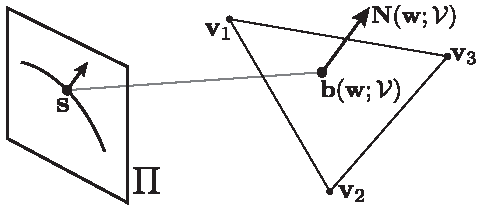
\includegraphics[width=3.33in]{projection2.pdf}
\caption{\label{fig:projection}  
\textbf{Silhouette projection terms.}
An observed silhouette point $\bs$ must correspond to a 3D point $\bb(\wpreimage, \cV)$ on the surface, parameterized by preimage coordinates $\wpreimage$, which include a triangle index and barycentric coordinates.  A ``smooth'' normal $\bN$ is computed at a surface point by Phong interpolation of vertex normals. This normal must lie on the contour generator for silhouette points, and the observed normal must be the projection of this normal.
}
\end{figure}

%.  stuff like this is fairly common in the NPR literature [Hertzmann and Zorin 2000], which the subtle difference that n dot v is  interpolated, rather than the normals.}

\paragraph{Point correspondences.}
The user also provides a few point correspondences on the animal, by
clicking image points in a simple UI.  A correspondence is a tuple $(i,t,\bc)$ indicating that vertex $\bv^t_i$ projects to a 2D point
$\bc$ in frame $t$, and the set of all correspondences is denoted $\cC$, with the restriction to frame $t$ being denoted $\cC_t = \{(i,\bc)|(i,t,\bc)\in\cC\}$.
This gives an energy
\begin{equation}
\E{point}^t(\cV_t) = \sum_{(i,_,\bc)\in\cC_t} || \bc - \bPi \bv_i^t ||^2
\label{eq:Epoint}
\end{equation}
These correspondences could also be detected automatically by a
feature matching algorithm. For the animals that we consider, these
correspondences are necessarily very sparse, as there are few good
corner features on them; they provide guidance for overall rigid
motion and for rotation. 

Summing the above terms ({\em sil, nrm, sil-smooth, point}) yields the data term $\E{data}^t(\cV_t, \cW_t)$.
%\begin{align}
%\E{data}^t =
% \w{sil} \E{sil}^t + \w{nrm} \E{nrm}^t(\cV_t) + \w{point} \E{point}^t(\cV_t)
%\end{align}

\subsection{Regularization terms}
The key to our regularization terms is in the choice of the deformation measures~$D$. We first describe the general form of the ARAP model, and then describe how it is applied to individual energy terms.

% \aron{I don't think any of the energies should have semicolons in the parameter lists.}  the semicolon separates 

\subsubsection{As-rigid-as-possible (ARAP) energy.}
\def\earap{E^\text{\sc{arap}}}
At various stages in the formulation, $\ED$ will take the form of an ARAP energy~\cite{Sorkine:2007:ARA}.  Let the pair of meshes to be compared be $\cV = \{\bv_i\}_{i=1}^n$ and $\cU = \{\bu_i\}_{i=1}^n$ and recall that all meshes have the same topology.  Then the ARAP energy is a measure of how ``different'' the two meshes are.
It is expressed in terms of per-vertex rotations $R_i$ applied to each vertex of $\cU$ in order to most closely align the one-ring of each vertex in $\cV$ to the corresponding
one-ring of $\cU$, and measures the residual error of this alignment.
The energy is zero if $\cU$ and $\cV$ are related by a rigid transformation, and increases as the transformation between the meshes becomes more nonrigid.
Formally, it is defined as the minimization 
\begin{multline}
\earap(\cV, \cU; A) =\\
 \min_{R_1,...,R_N} 
\sum_{i=1}^N \sum_{j\in\cN(i)} 
\bigl\| \left( \bv_i - \bv_j \right) - A R_i\left(\bu_i - \bu_j\right)\bigr\|^2
\label{eq:earap}
\end{multline}
%where the doubled edge set $\Edoubled \equiv \bigcup_{(i,j) \in \cE} \{(i,j),(j,i)\}$.
%\aron{defining doubled edge set seems unnecessary, esp. the way you've defined the edge set.  (maybe change the definition to say $(i,j)\in\cE$ \textbf{iff} there's an edge from i to j)}
Each vertex has an associated $3\times3$ rotation $R_i$ that are included in the optimization variables, parameterization using the exponential map as $R_i = \exp[\br_i]$
where $\exp[\cdot]$ converts from axis-angle form to a $3\times3$ matrix using the exponential map~\cite{Grassia00}.
The parameter $A$ is a $3\times3$ matrix which is the identity for standard ARAP, but will allow us to incorporate explicit global rotations and scales in our formulation. 
One convention we will need to introduce is a means of referring to the $R_i$ outside the optimization.  We can write a version of $\earap$ which names the rotation matrices, and omits the explicit minimization.   The rotation optimization variables are then considered to be added to the global list of unknowns. If $\cR$ is a set of rotations $\{R_i\}$ then write 
\def\earaptag{\hat{E}^\text{\sc{arap}}}
\def\Rtag#1{R^{\text{#1}}}
\def\cRtag#1{\cR_{\text{#1}}}
\begin{equation}
\earaptag(\cV, \cU, \cRtag{}; A) =\!\!\!\!
\sum_{i=1}^N \sum_{j\in\cN(i)} 
\bigl\| \left( \bv_i - \bv_j \right) - A \Rtag{}_i\left(\bu_i - \bu_j\right)\bigr\|^2
\label{eq:earaptag}
\end{equation}
We now treat the rotations $\cR$ as one of the free variables to be optimized together with the meshes, but this is equivalent, since $E = \min_{\cR} \hat{E}$.
Note that this does not imply any approximation or change to the minimization problem: for general $f_i$, we always have $\sum_{i=1}^n \min_{x_i} f_i(x_i) = \min_{x_1, ..., x_n} \sum_{i=1}^n f_i(x_i)$.

\subsubsection{ARAP motion energy.}
We enforce frame-to-frame consistency in an ARAP sense, defining the mesh deformation measure as an ARAP energy.   Thus \eqref{Emotion0} becomes
\begin{equation}
\E{motion}(\cV_{1..T}) = \sum_{t=2}^T \min_{\lambda_t} \earap(\cV_{t-1}, \cV_t; \lambda_t I_{3\times3}) 
\label{eq:Emotion}
\end{equation}
where the minimization over the $\lambda$s means that scale change from frame to frame is not penalized (it is managed by the instance-core terms below).
% \aron{$\alpha_t$'s missing subscripts \awf{well, not, because bound inside the summation, but ...}}

\subsubsection{ARAP core-template energy.}
The core-template energy is also expressed as ARAP, but with an additional small-rotation penalty.   Eq.~\eqref{Ecortpl0} becomes
\begin{multline}
\E{core-template}(\Vcore,\Vtemplate,\cRtag{core}) = \\
\earaptag(\Vcore, \Vtemplate, \cRtag{core}; I_{3\times3})
\label{eq:Ecortpl}
\end{multline}
introducing variables $\cRtag{core} = \{\Rtag{core}_i\}_{i=1}^N$.  Also defining the function $\angle(R)$ as the rotation angle of the matrix $R$, we introduce a regularizer on the rotation magnitude, given by
\begin{equation}
\E{core-template-reg}(\cRtag{core}) = \sum_{i=1}^N \angle(\Rtag{core}_i)^2
\label{eq:Ecortplreg}
\end{equation}

\subsubsection{``Hinted ARAP'' instance-core energy.} 
\label{sec:markup}
%\aaron{This section is long, complicated and important, so it deserves a more grand introduction and maybe more signposting. (Ideally, it would be a separate subsection, but that would break the organization.)}
% \aaron{"core-instance energy", for consistency with usage above.\awf{no, matches parameter ordering, and EArap not symmetric}}
The last of the deformation terms, from \eqref{Einscor0}, penalizes the deformation from core to instance.  We will again introduce explicit rotation variables, so \eqref{Einscor0} becomes
\begin{equation}
\E{instance-core}(\Vcore,\cV_{1..T},\cQ,\cG) = \sum_{t=1}^T \earaptag(\Vcore,\cV_t, \cQ_t;\alpha^G_t R^G_t)
\label{eq:Einscor}
\end{equation}
with new unknown rotation variables $\cQ_t = \{Q_i^t\}_{i=1}^N$, gathered across all frames in the list $\cQ = \{\cQ_t\}_{t=1}^T$.

This is an ARAP energy, but will now undergo important modifications in order to constrain the range of motion of the animal.
We find that allowing completely independent rotations for each vertex
provides too many degrees of freedom for the inherent depth
ambiguities of single-view fitting. In
particular, we observe limbs that twist and splay out of the image
plane, while still matching the silhouettes. 
In order to address this issue, we
introduce a novel scheme for restricting limb motion, based
on a lightweight, user-provided annotation of the mesh. The motion is separated into per-vertex motion, and global rotation, as described below.

\def\grparams{\boldsymbol\theta}
%\def\hintparam#1#2{\boldsymbol\gamma_{#1}^{#2}}
\def\hintparam#1#2{\boldsymbol\gamma_{{#1,#2}}}
When supplying an initial estimate of
the core geometry, the user places the mesh vertices into $M$ groups (\Figref{template}).  Each group $m$ has a set of group parameters $\grparams_m$.
Each vertex $i$ is assigned to a group $m(i)$,
the rotation $Q_i^t$ at frame $t$ for this vertex is parameterized by a lower-dimensional parameter vector $\hintparam it \in \mathbb R^{d_m}$.

The dimensionality $d_m \in \{0,1,3\}$ controls how freely the vertices in group~$m$ may deform.
%However, this representation is less restrictive than a skeleton model, because it still allows substantial
%deformations.  Even the \grp{rigid} groups (see below) allow some nonrigid
%deformation, although at an energy cost.
Three different group types are defined, depending on the dimensionality for that group:

$\bullet$ \grp{rigid} ($d_m=0$): Parts of the model which move near-rigidly, such as an animal's skull.  The group parameters comprise a rotation per frame, $\grparams_m = \{\bomegaa^1_m, \ldots, \bomegaa^T_m\} \subset \mathbb R^3$, and each vertex rotation is simply a copy of the group rotation $Q_i^t = \exp[\bomegaa^t_{m(i)}]$.

$\bullet$ \grp{nonrigid} ($d_m=3$): General non-rigid motion. Each vertex's rotation is unconstrained, so $Q_i^t = \exp[\hintparam it]$, and the group parameters are empty $\grparams_m = \{\}$. This is the normal ARAP case.

$\bullet$ \grp{hinge} ($d_m=1$): Components, such as animals' legs, which comprise mostly rigid components linked by coaxial hinges.  In this case, the group parameters are a single global (time-independent) rotation axis, $\grparams_m = \ba_m \in \mathbb R^3$, and each vertex is parameterized by a single scalar $\hintparam it \in \mathbb R$, so $Q_i^t = \exp[\hintparam it\ba_{m(i)}]$.
To see why this works, consider a mesh which comprises two rigid parts linked by a hinge joint.  Then if $\cU$ and $\cV$ are two instances of this mesh with the hinge in different positions, the minimum of the ARAP energy will be found when all vertices, both at the hinge and elsewhere, are associated with rotations sharing the hinge's axis.   
Each vertex in the group therefore rotates about a common axis, but with varying angle.  Note that this combats splaying within the legs, but does not inhibit correct splaying at the hips, for example when the dog turns in \Figref{teaser}.

%One may also use two degree-of-freedom components ($K_m=2$), though we have not found them useful in this work.
$\bullet$ \grp{pivot} ($d_m=2$): 
For completeness although we have not used them, \grp{pivot} components (named after pivot joints~\cite[page 64]{Grassia00}), have two degrees of freedom ($\hintparam it \in \mathbb R^2$).  The group parameters are $\grparams_m = \{\ba_m^1, \ba_m^2\}$, and the rotations are given by $Q_i^t = \exp[\hintparam i{t,1}\ba^1_{m(i)}]\exp[\hintparam i{t,2}\ba^2_{m(i)}]$.

% Note that for some group types, $\grparams_m$ is different for each $t$, for example the rigid basis for a head, and for others it is fixed for the entire sequence, for example the hinge basis for legs.

\subsubsection{Instance-core motion energy}
Having access to the ARAP rotations $\cQ$ in the optimization, we define an additional motion prior, as follows.
\begin{equation}
\E{instance-core-motion}(\cQ) = \sum_{t=2}^T \sum_{i=1}^N \angle( Q_i^t (Q_i^{t-1})^\top ) ^2
\label{eq:Einscormotion}
\end{equation}
This prior is typically used with a very low weight, but is useful to stabilize the optimization.

%This term also provides an implicit shape regularization.  Specifically, if we were to only regularize based on individual vertices (e.g., $\sum_t \| \bv_{i,t} - \bv_{i,t-1}\|^2$), then vertices far from measurements would be unconstrained.  \aaron{still unclear to me why this is a good way to resolve that.}

\subsubsection{Global per-frame rigid/camera transformation}
We also incorporate a per-frame rotation matrix and per-frame scaling to account for changes in camera zoom and object distance.  These quantities are parametrized by rotations $R^G_t$ and scales $\alpha^G_t$, gathered into a list of {\bf pose parameters}
\begin{equation}
\cG = \{\alpha^G_t, R^G_t\}_{t=1}^T
\end{equation}
Including global pose parameters is necessary for the hinted ARAP constraints on the body groups (\S\ref{sec:markup}) to be expressed in the core (local) coordinates. For example, the axis for leg rotations should always be transverse to the knees, even if the animal has turned relative to the camera.

In some cases, we also restrict the global rotation $R^G_t$, so it is parameterized by a parameter vector $\gamma^G_t$ with fewer than 3 degrees of freedom.  In cases where the animal moves in a straight path without turning, global rotations are around a single user-specified ``pitch'' axis, so $\gamma^G_t$ is 1-dimensional.  When the animal does turn, we often restrict the global rotation to two axes including yaw (heading) and pitch, but excluding roll.  Details on specific examples are given in the results (\S\ref{sec:results}).

\subsubsection{Smooth rigid/camera motion.} 
The velocity of the rigid/camera coordinates is penalized by
\begin{equation}
\E{camera-R-motion}(\cG) = \sum_{t=2}^T \angle(R^G_t (R^G_{t-1})^\top)^2
\end{equation}
Camera scale velocity is penalized by
\begin{equation}
\E{camera-scale-motion}(\cG) = \sum_{t=2}^T \left ( \log(\alpha^G_{t}) - \log(\alpha^G_{t-1}) \right )^2
\end{equation}
The log domain is used in order to prevent very small scales. 


% \subsubsection{Core shape prior.} 
% In some cases, parts of the shape can be unconstrained. For example,
% when observing a camel walk parallel to the image plane, we have no
% silhouette constraints on the interior shape. In order to resolve
% these ambiguities, we bias the core shape toward the input 
% (initialization) shape $\Vtemplate$, in an ARAP sense:
% \begin{equation}
% \E{core} = \earap(\Vcore, \Vtemplate; I).
% \label{eq:Ecore}
% \end{equation}
% This term is augmented by an additional regularizer, added to the minimization in~(\ref{eq:earap}), of the form 
% \begin{equation}
% 	\E{coreRot} = \sum_i ||\br_i ||^2
% 	\label{eq:EcoreRot}
% \end{equation}
% where the $\br_i$ here refer to the ARAP rotations in the computation of $\E{core}$.
% The core term is given a very small weight and has little or no effect,
% other than resolving ambiguities.

% We add a Laplacian regularization term to the core geometry, in order
% to encourage smooth shapes:
% \begin{equation}
% \E{Laplace} = \bar{\alpha}^2 \sum_i  \left\| \bv_i - \frac{1}{|\cN(i)|} \sum_{j
%     \in \cN(i)} \bv_j \right\|^2
% \end{equation}
% The term is weighted by the average scale 
% $\bar{\alpha} = \sum_t \alpha^G_t / T$ in order to prevent this term
% shrinking the core geometry to a point.





\section{Optimization Algorithm}
\label{sec:optimization}

The above energy function is a large-scale non-convex optimization
problem, and so both the choice of optimizer and initialization are
important.  The optimization alternates between different subsets of the unknowns.  Unless stated otherwise, each optimization step uses a large-scale Levenberg-Marquardt algorithm.  All gradients are computed semi-automatically through symbolic differentiation~\cite{Paprocki11} with manual fixup. Note that many terms (e.g., $w_j$ and $\bN_j$ in Eq.~\ref{eq:Enormals}) have complex dependencies on the unknowns, but liberal use of the chain rule keeps the code compact with only a small impact on efficiency.  Rotations are parameterized using the exponential map~\cite{Grassia00}.

As there are a large number of variables in the optimization (about 500,000 for the longest sequence)
and some of our test sequences approach 200 frames, we have implemented the optimization in ``sweeps,'' where each frame is visited sequentially, and only the energy terms relating to that frame are optimized.  

The shape in each frame is initialized as follows. The core geometry $\Vcore$ is initialized to the user-provided mesh $\Vtemplate$.  For the first sweep, an important task is to ensure reasonable initialization of the preimages $\cW$.  To this end, 
several weights are zeroed ($\w{sil} = \w{nrm} = \w{sil-smooth} = 0$) and the core is fixed ($\w{core-template-reg} = \w{core-template} = \infty$).  Then a sequence of optimizations is performed with $T$ increasing from 1, varying only $\cV_T$ at each step.

The algorithm then resets the weights to their default values, and each sweep alternates the following updates:
\begin{enumerate}
\item Optimize the core geometry $\Vcore$ and all local and global pose variables ($\cG, \cRtag{core}, \cQ_t$), holding all other variables fixed.
\item Optimize all preimage coordinates $\cW_t$, holding the other variables fixed, using dynamic programming~\cite{Cashman:2012:WSA}.
\item Jointly optimize instance geometry ($\cV_t$), scale ($\alpha^G_t$), and preimages ($\cW_t$), holding other variables fixed. 
%This is done in a forward sweep over frames (e.g., optimizing frame $t$, holding frames $t-1$ and $t+1$  fixed\awf{check $t+1$ still used}).  
In our current implementation $\w{sil-smooth}$ is zeroed for this step, due to the expense of recomputing geodesic distances which yields some jitter in the contour generators.   It would be interesting future work to look at approximations to ameliorate this.
\end{enumerate}
We typically run for 20 sweeps, although the instance variables are generally close to their final values after 5 sweeps.

\awf{
Note that as many of our energy terms are quadratic, there are ``closed form'' solutions to some of the subproblems.    However, it is almost certainly not worthwhile to exploit those: running the Levenberg Marquardt algorithm on a quadratic problem will not be more than say 2x slower than a quadratic solver, and running LM on a problem which admits quadratic alternations will almost certainly be quicker~\cite{Buchanan05}.
}


\section{Results}
\label{sec:results}

\begin{figure}
\begin{center}
\includegraphics[height=32mm]{figures/fig1-template-camel.png}~
\includegraphics[height=32mm]{figures/fig1-template-impala.png}~~~
\includegraphics[ width=32mm,angle=90]{figures/fig1-template-fish.png}
\end{center}
\caption{\textbf{Templates for camel, impala, and fish.}  Motion domains for the camel and impala are as for the dog, but the camel's neck is of type \grp{hinge}.  The fish is all of type \grp{nonrigid}.}
\label{fig:templates}
\vspace{-4mm}
\end{figure}

We demonstrate our method on video sequences of three mammals (dog, camel, impala) and a fish (sea bass), all obtained from the stock photography site shutterstock.com.  Template meshes (\Figref{templates}) were obtained by downloading appropriate-looking meshes from turbosquid.com, except for the dog, where we deliberately chose an ill-fitting mesh in order to show that the output is not strongly tied to the template.

All runs used the weights $\w{core-template-reg} = 8192, \w{motion} = 0.5, \w{point} = 2$, and all used customized camera motion weights: high for the impala and camel, where the camera is fairly static, low for the dog and fish.
Then the impala, fish, and camel shared all but one weight: $\w{sil-smooth}$ which was $4$ for the fish, $10$ for the others.  The dog has a different weight vector because it is the only model for which $\w{instance-core-motion}$ is nonzero.  Computation times were all of the order of 5-20 minutes per sweep, with sequences requiring from 5-20 sweeps.

\begin{figure}
\setlength{\awfw}{0.25\linewidth}
\def\awfig#1{\includegraphics[width=\awfw]{#1}}
\def\awfp#1#2#3{%
\parbox{\awfw}{%
\awfig{vid/impala0/Impala_1_Reduced_3B_AreaWeightedNormals_85-184_User_Constraints_Cropped/#2.png}\\
\awfig{vid/impala0/Impala_1_Reduced_3B_AreaWeightedNormals_85-184_Segmentations_Cropped/shutterstock_v1981186_1_1_00#3#2.png}\\
\awfig{vid/impala0/Impala_1_Reduced_3B_AreaWeightedNormals_85-184_10,1,1e-3,0.5,2,5e-2,0,0,0,8192,1024,0,0.5,8192_1.0,32.0,32.0,64.0,32.0_Cropped/#1/0.png}\\
\awfig{vid/impala0/Impala_1_Reduced_3B_AreaWeightedNormals_85-184_10,1,1e-3,0.5,2,5e-2,0,0,0,8192,1024,0,0.5,8192_1.0,32.0,32.0,64.0,32.0_Cropped/#1/2.png}}}
\awfp{40}{125}{}%
\awfp{50}{135}{}%
\awfp{60}{145}{}%
\awfp{70}{155}{}
\caption{\textbf{Leaping Impala.}  Four frames from a 100-frame sequence. \textbf{Top:} input frames with 15 point tracks.  \textbf{Row 2:} Silhouette masks.   Note that these can be imperfect.  \textbf{Row 3:} Overlaid 3D reconstruction. \textbf{Bottom:} Oblique view.}
\label{fig:impala}
\end{figure}

Visualizations and results are shown in the accompanying video, and in Figures \ref{fig:teaser}, \ref{fig:impala}, \ref{fig:fish}.  As can be seen in the examples, the method produces models which match the silhouette reasonably closely (although errors of up to 10 pixels do occur), and produces smooth meshes.   The video reveals that the mesh motion is mostly smooth, although the first order motion prior does allow some jitter.  It also has some difficulty correctly interpolating the motion of the dog's head when it is completely occluded by the body.   These effects might be repaired by a second order motion prior, but that is future work.

To investigate the behaviour of the energy weights, we varied two important parameters, $\w{instance-core}$ and $\w{core-template}$, through four orders of magnitude.  A high value of the core-template weight corresponds to ARAP fitting of the template to the sequence, and yields either overly rigid reconstructions, or allows too much variation in the instances.   Conversely, moderate values yield higher fidelity reconstructions, evidence of the value of the template-core-instance formulation.  Note that in this case, the impala template is visually very close to the subject's shape, but is different in proportion, so adapting the core still gives a more realistic model.

In order to test the benefit of ARAP as a deformation model for vision, we show comparisons with linear basis shapes \cite{Bregler:2000:RNR,Cashman:2012:WSA}.  To avoid implementing a completely different system, we simply fitted to our best impala model using PCA, and projected the recovered geometry onto the PCA basis.   As might be expected, large motions are poorly represented under the PCA model, as the side-by-side comparison in \Figref{linear} illustrates. 

%Note that this is a best case comparison for linear b
%\aaron{todo: finish this sentence? Note that this is a best-case-comparison for linear bases: direct attempts to apply previous methods on our data fail because...}  I decided not to say that cos it implies our solution is best


\begin{figure}[t]
\begin{center}
\vspace{-3mm}
\hspace{-10pt}\includegraphics[width=1.03\linewidth]{figures/3x3_parameter_settings_annotated.png}
\end{center}
\caption{\textbf{Effect of $\w{instance-core}$ and $\w{core-template}$ parameters.}  The parameters are varied through four orders of magnitude to investigate the effect of extreme settings. Left column: too small instance-core weight causes collapse along the viewing direction.}
\label{fig:parametergrid}
\end{figure}
\begin{figure*}
\begin{center}
\includegraphics[width=0.45\linewidth]{figures/lbs-comparison/34.png}~~~%
\includegraphics[width=0.45\linewidth]{figures/lbs-comparison/99.png}
\end{center}
\caption{\textbf{Comparison with linear basis shapes.} Each pair: left is our method, right is PCA of our solution. The range of motion of the impala means that even with eight PCA bases, as recovered by~\protect\cite{Cashman:2012:WSA}, significant errors remain in the linear model.
}
\label{fig:linear}
%\end{figure*}

%\begin{figure*}
\setlength{\awfw}{0.125\linewidth}
\def\awfig#1{\includegraphics[width=\awfw]{#1}}
\def\awfp#1{%
\parbox{\awfw}{%
\awfig{vid/fish/#1/0.png}\\
\awfig{vid/fish/#1/2.png}}}
\awfp{10}%
\awfp{20}%
\awfp{30}%
\awfp{40}%
\awfp{50}%
\awfp{60}%
\awfp{70}%
\awfp{80}
\caption{\textbf{Swimming sea bass.}  Frames from a 114-frame sequence.  Seven point tracks were used.   The sharp tail fin is recovered without any special modelling.}
\label{fig:fish}
\end{figure*}

\section{Discussion, Limitations, and Future Work}

This paper introduced a method for reconstructing time-varying 3D
geometry of animal movements. While much previous
work in computer graphics has focused on the use of specialized
capture equipment or studios, we instead work entirely from monocular
video; all our examples come from stock footage on the web.

A core technical contribution of our work is the use of ARAP as a prior
for articulated, non-rigid reconstruction. We show that ARAP can effectively model
articulation and non-rigid reconstruction. An alternative, that we
considered, would be to directly estimate a skinned, skeleton-based
rig from video data.
% (as has previously been done from 3D data, e.g., \cite{Jacobson:2012:FAS}). 
We chose the ARAP representation because we
believe that estimating a skeleton from data would be much more
difficult, requiring a combinatorial optimization, many local minima,
and difficult-to-specify user constraints. In contrast, the ARAP
formulation works with a straightforward optimization and relatively
few user constraints. We believe that it should be possible to learn
many of the variables that are currently user-specified, such as the
mesh clustering. However, both ARAP
and skeleton-based estimation are interesting avenues for future work.

Although our method requires user input, there is no provision made for interactive cleanup of the model: the user is assumed to be able to produce reasonably accurate silhouettes and point tracks.  However, for many sequences, one might imagine a user interface to adjust the model, and fast minimization to the new optimum would be necessary.
% A constraint that we have not included is volume preservation from frame to frame, which should be approximately satisfied 

Because we use silhouettes as our primary constraint, our method does
not estimate detailed shape, and often exhibits errors at internal
occluding contours. Moreover, we do not perfectly fit all
silhouettes. Estimating detailed shape would likely require fitting
texture and/or lighting, a challenging problem for future work. 

% Our method is presently limited to smooth structures; \awf{apparently not. creases on the fish work fine....}  handling sharp creases should be a straightforward extension.

\begin{figure*}
\setlength{\awfw}{0.16\linewidth}
\setlength{\fboxsep}{0pt}%
\setlength{\fboxrule}{1pt}%
\def\awfig#1{{\includegraphics[width=\awfw,trim=3cm 2cm 25mm 5cm, clip]{#1}}}
\def\awfp#1{%
\parbox{\awfw}{%
\awfig{vid/dog0/Boxer_0F_DOC_Cropped/#1/1.png}}}
\awfp{113}%
%\awfp{123}%
\awfp{133}%
\awfp{145}%
\awfp{151}%
\awfp{166}%
\awfp{176}%
%\awfp{195}
\caption{\textbf{Contour generator.}  The recovered preimage points $\cW_t$ at several frames of the dog sequence.  The contour generator moves across the mesh, indicating which parts of the shape are constrained by the data.}
\label{fig:cg}
\end{figure*}

\bibliographystyle{acmsiggraph}
\bibliography{arapsfm}
\end{document}

literature:

http://isg.cs.tcd.ie/cosulliv/Pubs/Skrba_CGF09.pdf




http://vision.eecs.ucf.edu/papers/cvpr2008/6.pdf
Reconstructing Non-stationary Articulated Objects in Monocular Video using Silhouette Information
   Deblur occupancy grid.   Dumb but a kernel of an idea in there if correctly reformulated.   Good only for 


Modeling with silhouettes...
